\documentclass[12pt, titlepage]{article}

\usepackage{booktabs}
\usepackage{tabularx}
\usepackage{hyperref}
\usepackage{float}
\hypersetup{
    colorlinks,
    citecolor=black,
    filecolor=black,
    linkcolor=red,
    urlcolor=blue
}
\usepackage{graphicx}
\usepackage[usenames, dvipsnames]{color}

\usepackage[round]{natbib}

\title{SE 3XA3: Requirements Document\\GrateBox}

\author{Team 8, Grate
		\\ Kelvin Lin (linkk4)
		\\ Eric Chaput (chaputem)
		\\ Jin Liu (liu456)
}

\date{\today}

%The follow 2 lines of code below were obtained from: 
%https://gitlab.cas.mcmaster.ca/ThisTooShallParse/3XA3_CParser/blob/master/Req_Update/L01_Group7_Requirements_Rev0.tex
\usepackage{mdframed}
\newmdenv[linecolor=black]{reqbox}


%% Comments

\usepackage{color}

\newif\ifcomments\commentstrue

\ifcomments
\newcommand{\authornote}[3]{\textcolor{#1}{[#3 ---#2]}}
\newcommand{\todo}[1]{\textcolor{red}{[TODO: #1]}}
\else
\newcommand{\authornote}[3]{}
\newcommand{\todo}[1]{}
\fi

\newcommand{\wss}[1]{\authornote{blue}{SS}{#1}}
\newcommand{\ds}[1]{\authornote{red}{DS}{#1}}
\newcommand{\mj}[1]{\authornote{red}{MSN}{#1}}
\newcommand{\cm}[1]{\authornote{red}{CM}{#1}}
\newcommand{\mh}[1]{\authornote{red}{MH}{#1}}

% team members should be added for each team, like the following
% all comments left by the TAs or the instructor should be addressed
% by a corresponding comment from the Team

\newcommand{\tm}[1]{\authornote{magenta}{Team}{#1}}


\begin{document}

\maketitle

\pagenumbering{roman}
\tableofcontents
\listoftables
\listoffigures

\begin{table}[h]
\caption{\bf Revision History}
\begin{tabularx}{\textwidth}{p{3.5cm}p{2cm}X}
\toprule {\bf Date} & {\bf Version} & {\bf Notes}\\
\midrule
October 7, 2016 & 1.0 & Started Functional Requirements\\
October 10, 2016 & 1.1 & Updated Functional Requirements\\
October 11, 2016 & 1.2 & Added Context Diagram\\
October 11, 2016 & 1.3 & Added Work Partitioning Table\\
October 11, 2016 & 1.4 & Added Off-the-Shelf Solutions\\
October 11, 2016 & 1.5 & Added to Non-Functional Requirements and Section 1\\
December 07, 2016 & 1.6 & Final Rev 1 Updates\\
\bottomrule
\end{tabularx}
\end{table}

\newpage

\pagenumbering{arabic}
\textcolor{RoyalPurple}{Purple text indicates changes made for Revision 1.}

\section{Project Drivers}

\subsection{The Purpose of the Project}

\subsubsection{Project Background}

Genetic algorithms serve as useful tools to search for near-optimal solutions to 
a wide variety of problems with incomplete or imperfect information by emulating 
the process of natural selection. The driving force for this project was the 
observed lack of genetic algorithm teaching tools. 

\subsubsection{Project Goals}

The primary goal of this project is to create a product that will teach users 
about the uses and theory behind genetic algorithms. The product must be 
engaging enough to maintain user interest while also bestowing them with 
practical knowledge about genetic algorithms. The success of this project will 
therefore be measured by both the engagement of the user and the increase in the 
user's practical knowledge of genetic algorithms.

\subsection{The Stakeholders}

\subsubsection{The Client}

The primary client of the Genetic Cars project is also the project's target 
audience, those with an academic interest in learning about genetic algorithms. 
This target audience is estimated to fall in the aged 16-24 student demographic. 
Since the Genetic Cars project does not have one formal client with whom to 
discuss the project's requirements, all project requirements are derived from 
the requirements of the project's target audience. These requirements were 
elicited via anonymous interviews with perspective users initially, however long 
term testing and user feedback shall serve to further specify and clarify 
requirements.

\subsubsection{The Customers}

The customers for the Genetic Cars project are the users outlined above. 
Assumptions about these user are listed in section 1.5.1 of this document.

\subsubsection{Other Stakeholders}

Other stakeholders for this project include:\\

-Testers: Those individuals who will aid in the testing of our product, by 
filling out surveys and providing feedback on the project. Significant crossover 
with our target audience for obvious reasons. Will provide the primary means of 
communication with our customers for this reason.\\

-Third-party technology experts: Those individuals who will help Grate learn 
about the technologies necessary for this project, as outlined in the design 
document and during team meetings. While not officially members of Grate, their 
aid will prove invaluable to learning the technologies necessary for this 
project to function, and they will be credited in final documentation.\\

-McMaster University library staff and faculty: Those individuals and services 
that will be interacted with to facilitate group meetings as outlined in the 
design document.

\subsection{Mandated Constraints}

\subsubsection{Scheduling Constraints}

This project shall adhere to the scheduling constrains outlined in below, with 
deliverables mandated to be completed by the dates outlined there.

\begin{tabular}{ p{6.7cm} l}

  Team Formation & Week of September 12\\

  Project Approval & Week of September 19\\

  Problem Statement & September 23\\

  Development Plan & September 30\\

  Requirements Document Revision 0 & October 7\\

  Proof of Concept Demonstration & Week of October 17\\

  Test Plan Revision 0 & October 28\\

  Design Document Revision 0 & November 11\\

  Revision 0 Demonstration & Week of November 14\\

  Lab Exercises & Throughout Term\\

  Final Demonstration (Revision 1) & Week of November 28\\

  Peer Evaluation of Other Team & Week of November 28\\

  Final Documentation (Revision 1) & December 8\\

\end{tabular}

\subsubsection{Budgetary and Technology Constraints}
This project shall not allow for the purchase of any third party product or 
service, as this project has no budget with which to acquire these. The product 
must also be compatible to technology that can be used freely by the users of 
the product without legal or monetary recourse.

\subsection{Naming Conventions and Terminology}

\textcolor{RoyalPurple}{Gene: A unit of heredity that is transferred from a parent to 
offspring and is 
held to determine some characteristic of the offspring. In this program a 'gene' 
will possess some variable of the car (number of wheels, size of each wheel, 
etc.) that is passed on to the next generation of car using genetic 
algorithms.}\\

\textcolor{RoyalPurple}{Population: The total amount of cars in the program. The genes 
available for the next generation are limited to the combinations of genes 
possible. Each car in the next generation is comprised of the genes of two cars 
in the population.}\\

\textcolor{RoyalPurple}{Sample: A portion drawn from a population, the study of which 
is intended to 
lead to statistical estimates of the attributes of the whole population.}\\

\textcolor{RoyalPurple}{Generation: The current iteration of cars in the program. Each 
new generation is composed of the mutation of the previous generation's 
genes.}\\

\textcolor{RoyalPurple}{Trait: A characteristic of the car determined by the genes a 
car possesses (i.e. the position of the wheels 
for one of the cars).}\\

\textcolor{RoyalPurple}{Attribute: Same as trait (used interchangeably with trait).}\\

\textcolor{RoyalPurple}{Mutate: To undergo or cause to undergo change in a gene or 
genes. This occurs after each generation of cars to varying extents determined 
by the mutation rate.}\\

\textcolor{RoyalPurple}{Mutation Rate: The rate at which mutations (seen above) occur. 
Can be varied in the program to increase or decrease the speed of convergence 
towards a more fit car.}\\

\textcolor{RoyalPurple}{Crossover: The exchange of genes between cars as part of how 
two cars reproduce in the program.}\\

\textcolor{RoyalPurple}{Reproduce: To produce a new car in a new generation by means of 
genetic propagation between two cars of the previous generation.}\\

\textcolor{RoyalPurple}{Random Seed: A number used to initialize a pseudorandom number 
generator. Will be used here to generate a pseudorandom member of the initial 
population for example.}\\

\subsection{Relevant Facts and Assumptions}

\subsubsection{User Assumptions}

The user base for this product consists of those wishing to learn more about 
genetic algorithms. It is assumed that this demographic consists primarily of 
secondary school and post-secondary students aged 16-24. This demographic is 
assumed to be very familiar with software applications and especially web-based 
software applications. This demographic is also assumed to have some preliminary 
background in both secondary school level evolutionary biology and basic 
mathematics. Finally, the users of this product are assumed to possess a level 
of maturity required to appreciate the academic portions of the product.

\subsubsection{Other Assumptions}

Grate assumes that all software tools listed in the development document will be 
available for use throughout the project. It is also assumed that the physics 
library being used is fully complete, although this assumption will be tested 
thoroughly throughout the lifetime of this project.

\newpage

\section{Functional Requirements}

\subsection{The Scope of the Work and the Product}

\subsubsection{The Context of the Work}
The following depicts a context diagram for Grate's Genetic Cars:

\begin{figure}[H]
  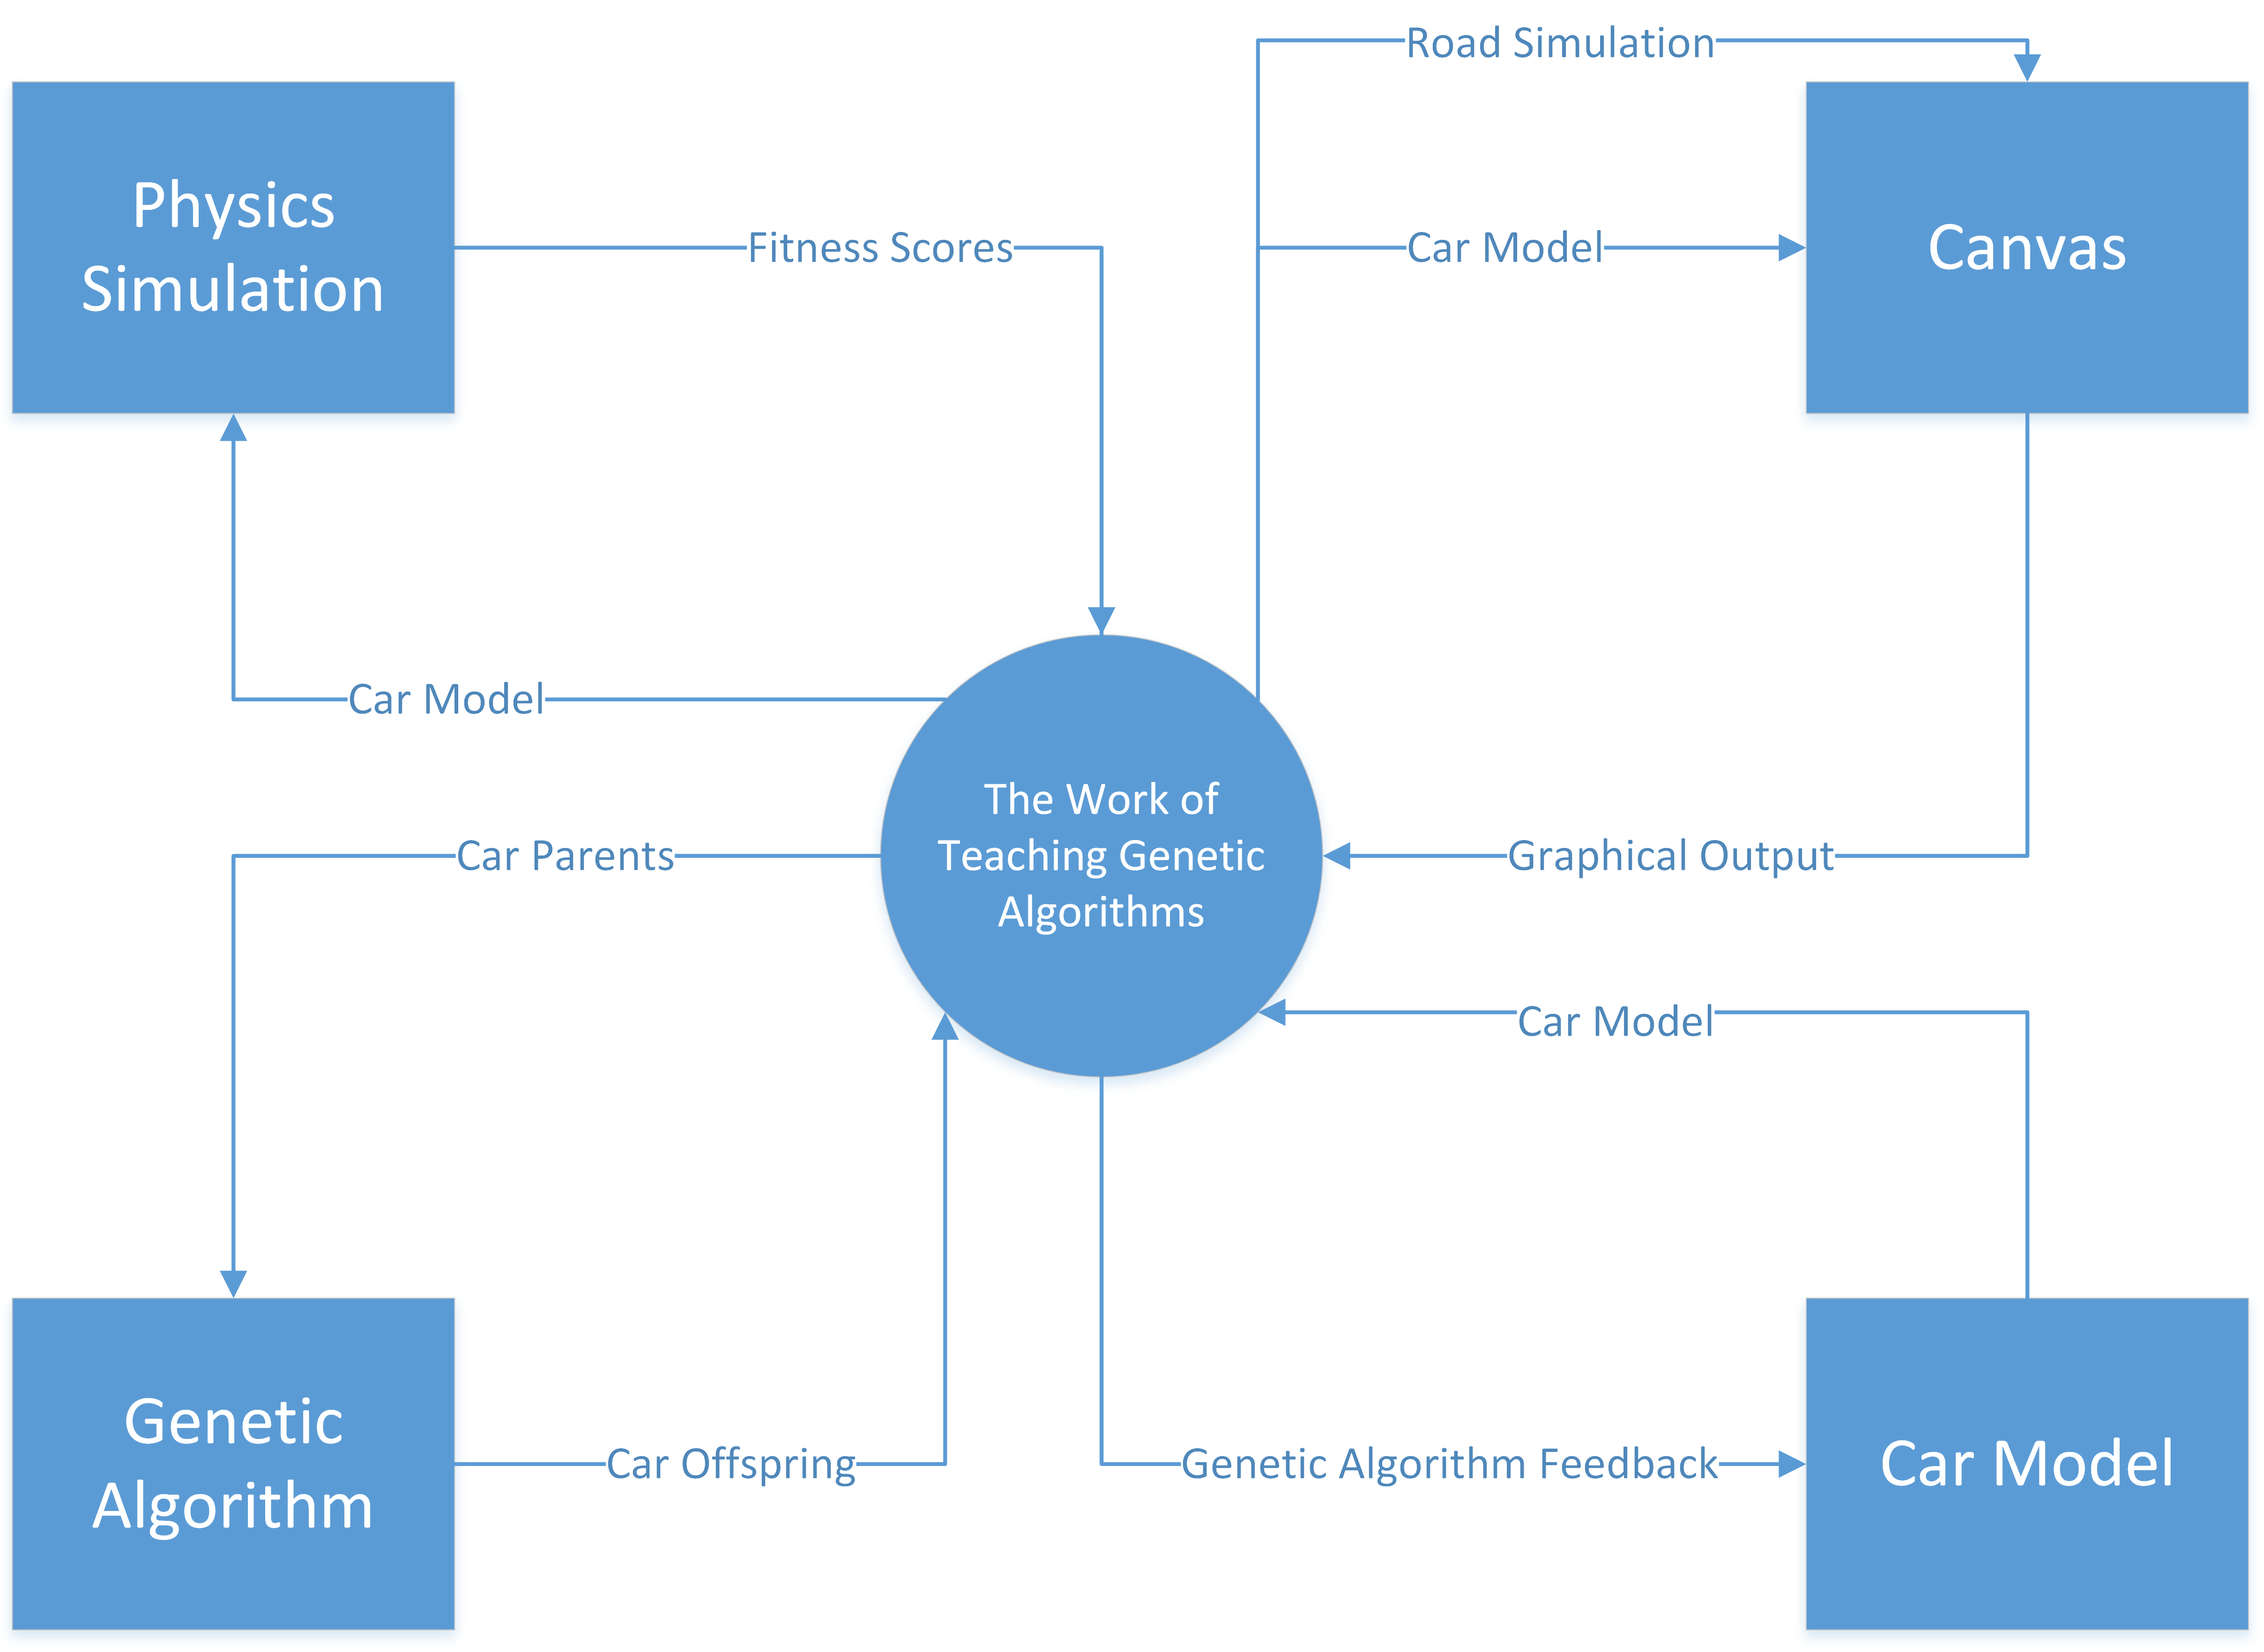
\includegraphics[scale=0.66]{ContextDiagram.png}
  \caption{The Context Diagram for Grate's Genetic Cars}
\end{figure}

\subsubsection{Work Partitioning}
\begin{table}[H]
\begin{tabularx}{\textwidth}{p{4cm}p{4cm}X}
\toprule {\bf Event Name} & {\bf Input and Output} & {\bf Summary}\\
\midrule
1. Physics Simulation simulates generation & Car Offspring (in), Fitness Scores 
(out) & Calculate parents for the next generation\\
& & \\
2. Canvas displays car results & Car model (in), Road simulation (in), Graphical 
Display (out) & Draw car model, Track top cars, Restart at the end of the 
generation\\
& & \\
3. Genetic algorithm generates new generation & Fitness Scores (in), Car 
Offspring (out) & Selects parents from fitness scores, Cross over genes, Mutate 
genes\\
\bottomrule
\end{tabularx}
\caption{\bf Work Partitioning Table}
\end{table}

\subsubsection{Individual Product Use Cases}
\begin{enumerate}

\item{Normal Operation}

\begin{itemize}
\item{User launches program.}
\item{The Genetic Algorithm generates a random seed.}
\item{The random seed is used to generate offspring using the default 
parameters.}
\item{The Physics Simulation takes the offspring (Car Model) and performs 
physics simulations to determine their fitness score.}
\item{The results are sent to the Canvas, which displays the results 
graphically.}
\item{The fitness scores are sent back to the Genetic Algorithm to generate new 
offspring.}
\end{itemize}

\item{User Modifies Any Parameter}
\begin{itemize}
\item{User launches program.}
\item{User modifies fields in the program that pertain to the Genetic 
Algorithm's attributes.}
\item{The Genetic Algorithm generates offspring based on the user's input.}
\item{The Physics Simulation takes the offspring (Car Model) and performs 
physics simulations to determine their fitness score.}
\item{The results are sent to the Canvas, which displays the results 
graphically.}
\item{The fitness scores are sent back to the Genetic Algorithm to generate new 
offspring.}
\end{itemize}

\end{enumerate}

\subsection{Functional Requirements}

%Box formatting template adapted from: 
%https://gitlab.cas.mcmaster.ca/ThisTooShallParse/3XA3_CParser/blob/master/Req_Update/L01_Group7_Requirements_Rev0.tex

%REQUIREMENT #1
\begin{reqbox}
	%
	\begin{tabular}{cc}
		Requirement \#: 1 & Requirement Type: Functional \\
	\end{tabular} \\
	%
	\textbf{Description:} \textcolor{RoyalPurple}{Each car must be composed of a car body 
with \textit{v} vertices and sides.} 
	\\
	\textbf{Rationale:}  \textcolor{RoyalPurple}{This requirement manages the complexity 
of the car model, 
	allowing for realistic distribution of traits among members of a population. 
	That is, this prevents large cars from being generated and using an excessive 
	amount of memory.} \\
	\textbf{Originator:} Kelvin Lin\\
	\textbf{Fit Criterion:} No car generated within population \textit{p} shall be 
	composed of more than \textit{v} vertices and sides.\\
	%  
	\textbf{Supporting Materials:} JavaScript \\
	\textbf{History:} Created October 7\textsuperscript{th}, 2016
	%
\end{reqbox}

\newpage

%REQUIREMENT #2
\begin{reqbox}
	%
	\begin{tabular}{cc}
		Requirement \#: 2 & Requirement Type: Functional \\
	\end{tabular} \\
	%
	\textbf{Description:} Each car may not have more than 
	\textit{number\_of\_vertices} wheels. \\
	\textbf{Rationale:}  The wheels must be attached to the car via a vertex 
between 
	two connecting vertices. This requirement ensures that no redundant or unused 
	wheels will be generated.\\
	\textbf{Originator:} Kelvin Lin\\
	\textbf{Fit Criterion:} No car generated within population \textit{p} shall be 
	composed of more than \textit{number\_of\_vertices} wheels.\\
	%  
	\textbf{Supporting Materials:} JavaScript \\
	\textbf{History:} Created October 7\textsuperscript{th}, 2016
	%
\end{reqbox}

%REQUIREMENT #3
\begin{reqbox}
	%
	\begin{tabular}{cc}
		Requirement \#: 3 & Requirement Type: Functional \\
	\end{tabular} \\
	%
	\textbf{Description:} The radius of each wheel must be at most \textit{r} 
units. 
	\\
	\textbf{Rationale:}  This requirement manages the complexity of the car model, 
	allowing for realistic distribution of traits among members of a population. 
	That is, cars with unrealistically sized wheels will not be generated.\\
	\textbf{Originator:} Kelvin Lin\\
	\textbf{Fit Criterion:} No cars generated will have wheels with a radius larger 
	than \textit{r}.\\
	%  
	\textbf{Supporting Materials:} JavaScript \\
	\textbf{History:} Created October 7\textsuperscript{th}, 2016
	%
\end{reqbox}

\newpage

%REQUIREMENT #4
\begin{reqbox}
	%
	\begin{tabular}{cc}
		Requirement \#: 4 & Requirement Type: Functional \\
	\end{tabular} \\
	%
	\textbf{Description:} The center of each wheel generated must be attached to a 
	vertex formed by connecting sides of the polygon car body. \\
	\textbf{Rationale:}  Wheels cannot be floating on or around the car. This 
	requirement ensures visual coherency by requiring wheels to be attached to the 
	car model. Knowing the center of the wheel will also allow the physics engine 
to 
	calculate the torque and distance that the car travelled.\\
	\textbf{Originator:} Kelvin Lin\\
	\textbf{Fit Criterion:} Each wheel displayed on the screen is attached to a 
	vertex formed by connecting sides of the polygon car body.\\
	%  
	\textbf{Supporting Materials:} JavaScript \\
	\textbf{History:} Created October 7\textsuperscript{th}, 2016
	%
\end{reqbox}

%REQUIREMENT #5
\begin{reqbox}
	%
	\begin{tabular}{cc}
		Requirement \#: 5 & Requirement Type: Functional \\
	\end{tabular} \\
	%
	\textbf{Description:} The mass of each car must not be less than 
	\textit{min\_weight}. \\
	\textbf{Rationale:} In order to have realistic physical simulations of car 
	models, the mass of the car must have a lower limit. The lower limit will 
	guarantee the simulations to work as expected. \\
	\textbf{Originator:} Kelvin Lin\\
	\textbf{Fit Criterion:} The mass of any car models generated are greater than 
	\textit{min\_weight}.\\
	%  
	\textbf{Supporting Materials:} JavaScript \\
	\textbf{History:} Created October 10\textsuperscript{th}, 2016
	%
\end{reqbox}

\newpage

%REQUIREMENT #6
\begin{reqbox}
	%
	\begin{tabular}{cc}
		Requirement \#: 6 & Requirement Type: Functional \\
	\end{tabular} \\
	%
	\textbf{Description:} The mass of each car must not exceed 
\textit{max\_weight}. 
	\\
	\textbf{Rationale:} In order to have realistic physical simulations of car 
	models, the mass of each car must have an upper limit. An upper limit reduces 
	the possibility of type incompatibility with certain APIs. Additionally, it 
	ensures that the mass of each car is encoded using a known number of bits.\\
	\textbf{Originator:} Kelvin Lin\\
	\textbf{Fit Criterion:} The mass of any car models generated do not exceed 
	\textit{max\_weight}.\\
	%  
	\textbf{Supporting Materials:} JavaScript \\
	\textbf{History:} Created October 10\textsuperscript{th}, 2016
	%
\end{reqbox}

%REQUIREMENT #7
\begin{reqbox}
	%
	\begin{tabular}{cc}
		Requirement \#: 7 & Requirement Type: Functional \\
	\end{tabular} \\
	%
	\textbf{Description:} The program shall display each generation of cars 
	traversing the road. \\
	\textbf{Rationale:} The purpose of this program is to show its users the 
effects 
	of genetic algorithms in an interesting and engaging manner. If the program did 
	not display each generation of cars traversing the road, then the program would 
	fail in accomplishing its original objective. \\
	\textbf{Originator:} Kelvin Lin\\
	\textbf{Fit Criterion:} Each generation of cars can be seen traversing a road 
on 
	the medium of output.\\
	%  
	\textbf{Supporting Materials:} JavaScript \\
	\textbf{History:} Created October 10\textsuperscript{th}, 2016
	%
\end{reqbox}

\newpage

%REQUIREMENT #8
\begin{reqbox}
	%
	\begin{tabular}{cc}
		Requirement \#: 8 & Requirement Type: Functional \\
	\end{tabular} \\
	%
	\textbf{Description:} The program shall display the fitness of the top 
	\textit{n} cars. \\
	\textbf{Rationale:} The ability to compare the performance of cars during each 
	generation is useful for observing the effects of genetic algorithms because it 
	shows the users the improvement and regression of the car's performance over 
	time.\\
	\textbf{Originator:} Kelvin Lin\\
	\textbf{Fit Criterion:} A medium of output exists to provide the fitness of the 
	car on the medium of display.\\
	%  
	\textbf{Supporting Materials:} JavaScript \\
	\textbf{History:} Created October 10\textsuperscript{th}, 2016
	%
\end{reqbox}

%REQUIREMENT #9
\begin{reqbox}
	%
	\begin{tabular}{cc}
		Requirement \#: 9 & Requirement Type: Functional \\
	\end{tabular} \\
	%
	\textbf{Description:} The program shall allow the user to enter a random seed 
to 
	generate cars from in lieu of a randomly generated seed. \\
	\textbf{Rationale:} The ability to enter a random seed allows the results of 
	cars to be compared and to be run on multiple computers: results are not lost 
as 
	a result of restarting the application. \\
	\textbf{Originator:} Kelvin Lin\\
	\textbf{Fit Criterion:} The user can input a random seed into the program 
	through an input device, and the random seed is used to dictate the random 
	behaviours of the program.\\
	%  
	\textbf{Supporting Materials:} JavaScript \\
	\textbf{History:} Created October 10\textsuperscript{th}, 2016
	%
\end{reqbox}

\newpage

%REQUIREMENT #10
\begin{reqbox}
	%
	\begin{tabular}{cc}
		Requirement \#: 10 & Requirement Type: Functional \\
	\end{tabular} \\
	%
	\textbf{Description:} The user shall be allowed to modify the mutation rate, 
	\textit{mutation\_rate}. \\
	\textbf{Rationale:} Allowing the users to modify the mutation rate allows the 
	program to fulfil its objective by showing the users how the mutation rate can 
	impact the performance of the cars. \\
	\textbf{Originator:} Kelvin Lin\\
	\textbf{Fit Criterion:} The user can input a mutation rate into the program 
	through an input device, and the mutation rate is used to produce offspring in 
	the program.\\
	%  
	\textbf{Supporting Materials:} JavaScript \\
	\textbf{History:} Created October 10\textsuperscript{th}, 2016
	%
\end{reqbox}

%REQUIREMENT #11
\begin{reqbox}
	%
	\begin{tabular}{cc}
		Requirement \#: 11 & Requirement Type: Functional \\
	\end{tabular} \\
	%
	\textbf{Description:} The user shall be allowed to change the number of cars 
per 
	generation \textit{s} in lieu of the default value. \\
	\textbf{Rationale:} Allowing the user to change the number of cars per 
	generation \textit{s} will allow the user to see how the size of a generation 
	affects the genetic algorithm. \\
	\textbf{Originator:} Kelvin Lin\\
	\textbf{Fit Criterion:} \textit{s} is equal to the user's input for every 
	generation produced by the program.\\
	%  
	\textbf{Supporting Materials:} JavaScript \\
	\textbf{History:} Created October 10\textsuperscript{th}, 2016
	%
\end{reqbox}

\newpage

%REQUIREMENT #12
\begin{reqbox}
	%
	\begin{tabular}{cc}
		Requirement \#: 12 & Requirement Type: Functional \\
	\end{tabular} \\
	%
	\textbf{Description:} The road generated must be the same across all 
	generations. \\
	\textbf{Rationale:} Using the same road for each generation allows for 
	comparability of performance between each generation. That is, since every car 
	will traverse the same course, their fitness and performance can be compared. 
\\
	\textbf{Originator:} Kelvin Lin\\
	\textbf{Fit Criterion:} The road for all simulations is the same. \\
	%  
	\textbf{Supporting Materials:} JavaScript \\
	\textbf{History:} Created October 10\textsuperscript{th}, 2016
	%
\end{reqbox}

%REQUIREMENT #13
\begin{reqbox}
	%
	\begin{tabular}{cc}
		Requirement \#: 13 & Requirement Type: Functional \\
	\end{tabular} \\
	%
	\textbf{Description:} The product must generate at least \textit{s} car samples 
	per generation. \\
	\textbf{Rationale:}  GAs improve by having a large number of samples 
	(representing members in a population) intermix traits. This requirement allows 
	the GA to work by guaranteeing that a sufficient sample will be present at all 
	times.\\
	\textbf{Originator:} Kelvin Lin\\
	\textbf{Fit Criterion:} Given a user generated input, \textit{s}, the program 
	should generate \textit{s} cars for each generation.\\
	%  
	\textbf{Supporting Materials:} JavaScript \\
	\textbf{History:} Created October 7\textsuperscript{th}, 2016
	%
\end{reqbox}

\newpage

%REQUIREMENT #14
\begin{reqbox}
	%
	\begin{tabular}{cc}
		Requirement \#: 14 & Requirement Type: Functional \\
	\end{tabular} \\
	%
	\textbf{Description:} The number of cars per generation \textit{s} shall not 
	exceed \textit{max\_cars\_per\_gen}. \\
	\textbf{Rationale:} Having a maximum number of cars per generation prevents 
	memory overflow from generating too many cars per generation.\\
	\textbf{Originator:} Kelvin Lin\\
	\textbf{Fit Criterion:} The number of cars generated per generation does not 
	exceed \textit{max\_cars\_per\_gen}.\\
	%  
	\textbf{Supporting Materials:} JavaScript \\
	\textbf{History:} Created October 10\textsuperscript{th}, 2016
	%
\end{reqbox}

%REQUIREMENT #15
\begin{reqbox}
	%
	\begin{tabular}{cc}
		Requirement \#: 15 & Requirement Type: Functional \\
	\end{tabular} \\
	%
	\textbf{Description:} The program shall use the top \textit{t} cars to generate 
	offsprings. \\
	\textbf{Rationale:} The number of cars allowed to reproduce needs to be 
	specified; otherwise, no improvement can be made in car performance over the 
	generations. \\
	\textbf{Originator:} Kelvin Lin\\
	\textbf{Fit Criterion:} The parent cars of the offspring are within the top 
	\textit{t} cars.\\
	%  
	\textbf{Supporting Materials:} JavaScript \\
	\textbf{History:} Created October 10\textsuperscript{th}, 2016
	%
\end{reqbox}

\newpage

%REQUIREMENT #16
\begin{reqbox}
	%
	\begin{tabular}{cc}
		Requirement \#: 16 & Requirement Type: Functional \\
	\end{tabular} \\
	%
	\textbf{Description:} The top \textit{t} cars shall not exceed \textit{t\_max}. 
	\\
	\textbf{Rationale:} This restriction prevents \textit{t} from exceeding 
	\textit{s} or take on an unreasonable value. It ensures that the program can 
	always run by setting an upper limit to the number of cars that can reproduce 
in 
	a given generation. \\
	\textbf{Originator:} Kelvin Lin\\
	\textbf{Fit Criterion:} The number of cars to choose from during reproduction 
	does not exceed \textit{t\_max}.\\
	%  
	\textbf{Supporting Materials:} JavaScript \\
	\textbf{History:} Created October 10\textsuperscript{th}, 2016
	%
\end{reqbox}

%REQUIREMENT #17
\begin{reqbox}
	%
	\begin{tabular}{cc}
		Requirement \#: 17 & Requirement Type: Functional \\
	\end{tabular} \\
	%
	\textbf{Description:} The top \textit{t} cars shall not be less than 
	\textit{t\_min}. \\
	\textbf{Rationale:} This requirement ensures that there will be a sufficient 
	number of cars to produce offspring in the subsequent generations. \\
	\textbf{Originator:} Kelvin Lin\\
	\textbf{Fit Criterion:} In each generation, there are at least \textit{t\_min} 
	parents to generate offspring.\\
	%  
	\textbf{Supporting Materials:} JavaScript \\
	\textbf{History:} Created October 10\textsuperscript{th}, 2016
	%
\end{reqbox}

\newpage

%REQUIREMENT #18
\begin{reqbox}
	%
	\begin{tabular}{cc}
		Requirement \#: 18 & Requirement Type: Functional \\
	\end{tabular} \\
	%
	\textbf{Description:} A car that stalls for more than \textit{max\_secs} shall 
	be deemed non-moving. \\
	\textbf{Rationale:} A time limit needs to be imposed on the simulations in 
order 
	to prevent the cars from running indefinitely without making progress. \\
	\textbf{Originator:} Kelvin Lin\\
	\textbf{Fit Criterion:} All cars that say in the same spot for 
	\textit{max\_secs} are marked as non-moving and the simulation for that car is 
	stopped.\\
	%  
	\textbf{Supporting Materials:} JavaScript \\
	\textbf{History:} Created October 10\textsuperscript{th}, 2016
	%
\end{reqbox}

%REQUIREMENT #19
\begin{reqbox}
	%
	\begin{tabular}{cc}
		Requirement \#: 19 & Requirement Type: Functional \\
	\end{tabular} \\
	%
	\textbf{Description:} The fitness of a car shall not be calculated until a car 
	is deemed to be non-moving. \\
	\textbf{Rationale:} The fitness of a car is determined by distance it moves 
	during the simulation, and the simulation runs while the car is moving. 
	Therefore, the fitness of a car cannot be determined until the car is 
	non-moving. \\
	\textbf{Originator:} Kelvin Lin\\
	\textbf{Fit Criterion:} After a car is deemed non-moving, it's fitness value 
can 
	be assessed.\\
	%  
	\textbf{Supporting Materials:} JavaScript \\
	\textbf{History:} Created October 10\textsuperscript{th}, 2016
	%
\end{reqbox}


%REQUIREMENT #20
\begin{reqbox}
	%
	\begin{tabular}{cc}
		Requirement \#: 20 & Requirement Type: Functional \\
	\end{tabular} \\
	%
	\textbf{Description:} The user shall be able to specify \textit{t} in lieu of 
	the default value. \\
	\textbf{Rationale:} This will allow users to see the effect of changing the 
	selectivity of the genetic algorithm. \\
	\textbf{Originator:} Kelvin Lin\\
	\textbf{Fit Criterion:} In each generation, \textit{t} cars are chosen to 
	generate offspring. \\
	%  
	\textbf{Supporting Materials:} JavaScript \\
	\textbf{History:} Created October 10\textsuperscript{th}, 2016
	%
\end{reqbox}

\newpage

\section{Non-functional Requirements}

\subsection{Look and Feel Requirements}

As discussed in section 1.2 of this document, the users of this product include 
students and others interested in learning about genetic algorithms. With this 
in mind, the Genetic Cars project must be accessible to those without a 
background in mathematics or computer science. This accessibility begins with 
the look and feel of the project. The Genetic Cars project should appear 
aesthetically pleasing while still presenting its functions in as clean a manner 
as possible.

\subsubsection{Appearance Requirements}

\begin{reqbox}
%
\begin{tabular}{cc}
Requirement \#: 21 & Requirement Type: Non-Functional \\
\end{tabular} \\
%
\textbf{Description:} The product shall be attractive to a student audience. \\
\textbf{Rationale:}  Part of the learning process is maintaining the attention 
of the users of the product. If users do not want to look at the product, it 
will be impossible to teach them anything.\\
\textbf{Originator:} Eric Chaput\\
\textbf{Fit Criterion:} A sampling of respective users shall, without prompting 
or enticement, be able to comprehend and use the product within sixty seconds of 
their first encounter with it. This same sampling shall also rate the appearance 
of the product on a scale from 1 to 10, and this rating shall be used to 
evaluate the requirement.\\
%  
\textbf{Supporting Materials:} JavaScript \\
\textbf{History:} Created October 7\textsuperscript{th}, 2016
%
\end{reqbox}

\newpage

\subsubsection{Style Requirements}

\begin{reqbox}
%
\begin{tabular}{cc}
Requirement \#: 22 & Requirement Type: Non-Functional \\
\end{tabular} \\
%
\textbf{Description:} The product shall appear inviting, educational, and 
professional. \\
\textbf{Rationale:}  If users do not believe our product contains a certain 
style, they will not respect it, and therefore, they will not use it.\\
\textbf{Originator:} Eric Chaput\\
\textbf{Fit Criterion:} 60\% of representative users shall agree that they feel 
they would want to use the product based on the professional and inviting style 
it contains. This majority should also agree that they can trust the product.\\
%  
\textbf{Supporting Materials:} JavaScript \\
\textbf{History:} Created October 7\textsuperscript{th}, 2016
%
\end{reqbox}

\subsection{Usability and Humanity Requirements}

\subsubsection{Ease of Use Requirements}
\begin{reqbox}
%
\begin{tabular}{cc}
Requirement \#: 23 & Requirement Type: Non-Functional \\
\end{tabular} \\
%
\textbf{Description:} The product shall be easy for anybody over the age of 6 to 
use. The product shall make the user want to use it and to show the product to 
their friends/family/etc.. The product shall be used by people with no training 
or education except for a basic knowledge of the English language and the most 
very basic functions of a computer, such as how to navigate to a web-site and 
how to enter inputs when prompted to do so. \\
\textbf{Rationale:}  In order for our product to reach a wide audience, it must 
be usable by a wide audience.\\
\textbf{Originator:} Eric Chaput\\
\textbf{Fit Criterion:}50\% of users 
shall be able to successfully complete a given set of tasks with the product 
within a specified period of time to be determined at the time of the sample. 
The representative sample shall also show a willingness to show the product to 
others.\\
%  
\textbf{Supporting Materials:} JavaScript \\
\textbf{History:} Created October 7\textsuperscript{th}, 2016
%
\end{reqbox}


\subsubsection{Personalization Requirements}

\begin{reqbox}
%
\begin{tabular}{cc}
Requirement \#: 24 & Requirement Type: Non-Functional \\
\end{tabular} \\
%
\textbf{Description:} The product shall allow the user to make simple 
adjustments to the product to 
allow for a variable length and amount of trials depending on user input.  \\
\textbf{Rationale:}  Interactivity is key to the learning process. The more 
interactive a product is the more likely a user is to maintain interest in it.\\
\textbf{Originator:} Eric Chaput\\
\textbf{Fit Criterion:}A simple check can be made to see if this possible.\\
%  
\textbf{Supporting Materials:} JavaScript \\
\textbf{History:} Created October 7\textsuperscript{th}, 2016
%
\end{reqbox}

\subsubsection{Learning Requirements}

\begin{reqbox}
%
\begin{tabular}{cc}
Requirement \#: 25 & Requirement Type: Non-Functional \\
\end{tabular} \\
%
\textbf{Description:} The product shall be easy for an intended user of the 
product to learn. The 
product shall be able to be used by these users with no training before use.  \\
\textbf{Rationale:}  The user should be focusing on learning about genetic 
algorithms, not on learning how to use the product.\\
\textbf{Originator:} Eric Chaput\\
\textbf{Fit Criterion:}50\% of users shall be able to successfully complete a 
given 
set of tasks with the product within a specified period of time to be determined 
at the time of the sample.\\
%  
\textbf{Supporting Materials:} JavaScript \\
\textbf{History:} Created October 7\textsuperscript{th}, 2016
%
\end{reqbox}

\newpage

\subsection{Performance Requirements}

\subsubsection{Speed and Latency Requirements}

\begin{reqbox}
%
\begin{tabular}{cc}
Requirement \#: 26 & Requirement Type: Non-Functional \\
\end{tabular} \\
%
\textbf{Description:}The response time of the product shall be fast enough to 
avoid a loss of 
interest by the user following an input, which shall be a period of time no 
longer then five seconds. The initialization of the product shall be rapid.  \\
\textbf{Rationale:}  The user should be focusing on learning about genetic 
algorithms, not on waiting to use the product.\\
\textbf{Originator:} Eric Chaput\\
\textbf{Fit Criterion:}Initialization shall be no longer then one minute. A 
majority representation of users shall be surveyed about the reaction time and 
requested to label their satisfaction with this time on a scale from one to ten. 
This survey data will then be analysed for feedback.\\
%  
\textbf{Supporting Materials:} JavaScript \\
\textbf{History:} Created October 7\textsuperscript{th}, 2016
%
\end{reqbox}

\subsubsection{Precision and Reliability Requirements}

\begin{reqbox}
%
\begin{tabular}{cc}
Requirement \#: 27 & Requirement Type: Non-Functional \\
\end{tabular} \\
%
\textbf{Description:}The product shall always converge towards a more optimal 
car. The product shall achieve near-optimal uptime. The product's numerical 
values shall be accurate.  \\
\textbf{Rationale:}  A learning product that is not accurate and reliable will 
not be taken seriously.\\
\textbf{Originator:} Eric Chaput\\
\textbf{Fit Criterion:}The product shall achieve 99 percent uptime. The product 
display of numerical values shall be accurate to two decimal places.\\
%  
\textbf{Supporting Materials:} JavaScript \\
\textbf{History:} Created October 7\textsuperscript{th}, 2016
%
\end{reqbox}

\newpage

\subsubsection{Longevity Requirements}

\begin{reqbox}
%
\begin{tabular}{cc}
Requirement \#: 28 & Requirement Type: Non-Functional \\
\end{tabular} \\
%
\textbf{Description:}The product shall be easy to update and upgrade following 
its initial public 
release.\\
\textbf{Rationale:}  Long term sustainability will allow our product to reach 
more people over time.\\
\textbf{Originator:} Eric Chaput\\
\textbf{Fit Criterion:}The creation of the product will consist of a series of 
updates, so Grate shall determine by internal surveys the difficulty of updating 
the product.\\
%  
\textbf{Supporting Materials:} JavaScript \\
\textbf{History:} Created October 7\textsuperscript{th}, 2016
%
\end{reqbox}

\subsection{Operational and Environmental Requirements}

The Genetic Cars project does not possess any operational and environmental 
requirements of note.

\subsection{Maintainability and Support Requirements}

See longevity requirements (Section 3.3.3) for more on this.

\subsection{Security Requirements}

This product requires no disclosure of sensitive information by either the user 
or the software program itself so there are no security requirements beyond what 
one would expect of any software program.

\subsection{Cultural Requirements}

This product requires no tailoring to meet specific cultural needs so that are 
no cultural requirements beyond what one would expect of any software program.

\subsection{Legal Requirements}

The Genetic Cars project does not possess any legal requirements of note as 
licensing is a non-issue for this project.

\subsection{Health and Safety Requirements}

\textcolor{RoyalPurple}{The Genetic Cars project does not possess any Health and Safety 
requirements beyond those outlined in section 4.3.3. under potential user 
problems.}

\section{Project Issues}

\subsection{Open Issues}
All open issues resolved.

\subsection{Off-the-Shelf Solutions}

\subsubsection{Ready-Made Product}
Similar solutions to Grate's Genetic Cars already exists, notably BoxCar2D 
(boxcar2d.com/) and Rednuht's Genetic Cars (rednuht.org/genetic\_cars\_2/). Both 
products demonstrate the effect of genetic algorithms through evolving cars by 
selecting for the longest distance travel. They differ in that BoxCar2D displays 
one car at a time, whereas Rednuht's Genetic Cars displays all of the cars in 
one generation at once. They both allow users to adjust parameters of the 
genetic algorithm in order to observe the effects of the algorithm. They both 
show the performance of the cars over time.

\subsubsection{Reusable Components}
The Box2D API and the D3 API can both be reused in Grate's Genetic Cars. The 
Box2D API provides functionality such as Vectors and Polygons that can be used 
to model the car. The D3 API provides visualization functionality that can be 
used to visualize the performance of cars over time. These APIs provide 
functionality external to the core functionality of Grate's Genetic Cars, which 
will make them valuable assets as Grate will not have to reimplement these APIs.

\subsubsection{Products That Can Be Copied}
Rednuht's Genetic Cars is licensed under the author's custom license which 
grants others the right to reuse his code as part of their solution. 
Furthermore, both BoxCar2D and Rednuht's Genetic Cars have released their 
algorithms in some form: BoxCar2D through visuals and text, and Rednuht's 
Genetic Cars through source code. Grate's Genetic Cars can draw inspiration from 
these sources in implementing a new innovative solution to teaching genetic 
algorithms.

\subsection{New Problems}

\subsubsection{Effects on the Current Environment}
\textcolor{RoyalPurple}{The program is accessed through a website and has no effects on 
the current environment. Therefore this is not applicable for this project.}

\subsubsection{Effects on the Installed Systems}
\textcolor{RoyalPurple}{This program is accessed through a website and is not 
installed. Therefore this is not applicable for this project.}

%Motivated by Nintendo's Health and Safety Documentation for the Nintendo 3DS 
%XL: 
%http://www.nintendo.com/consumer/info/en_na/docs.jsp?menu=3ds&submenu=ctr-doc-health-safety
\subsubsection{Potential User Problems}
Users may experience fatigue from prolong use of the product. Symptoms of 
fatigue can include eyestrain, dizziness, nausea, muscle pain, or general 
discomfort \citep{nintendo}. To prevent fatigue, users should take periodic 
breaks when using the 
program for prolonged periods of time \citep{nintendo}. However, fatigue should 
not pose a 
significant risk for this project, as the target audience for Grate's Genetic 
Cars is older teenagers and adults who have prior experience using computers and 
are  knowledgeable about the health concerns associated with prolong use of 
computers.

Users with epilepsy or prior history of seizures may also experience seizures or 
blackouts while using the product \citep{nintendo}. Symptoms of seizures may 
include convulsions, 
eye or muscle twitching, loss of awareness, altered vision, involuntary 
movements, and disorientation \citep{nintendo}. However, this risk is not 
significant as the risk 
of having a seizure from light flashes or patterns is low (about 1 in 4000), and 
the likelihood of experiencing a seizure can be reduced through simple steps 
\citep{nintendo}. 
Users can reduce the risk of experience seizures while using the product if they 
sit or stand away from the screen, use the smallest screen possible, use the 
product in a well lit room, take frequent breaks, and refrain from using the 
product if tired \citep{nintendo}.

\subsubsection{Limitations in the Anticipated Implementation Environment that 
May Inhibit the New Product}
Not applicable for this project.

\subsubsection{Follow-up Problems}
The implementation environment may become depreciated before the completion of 
the project, and the platforms the product is built for may no longer support 
the product after completion of implementation. This is a significant risk as 
modern programming languages and operating platforms are constantly evolving; 
however, this risk can be mitigated through writing maintainable code that can 
be converted to new standards as they arise.

\subsection{Tasks}
\subsubsection{Project Planning}
The V-Model of Software Development will be used in the development of this 
project. The V-Model to be followed is depicted below:

%The following figure was adapted from Dr. Smith's Lecture 5 Slides, available 
%at 
%https://gitlab.cas.mcmaster.ca/smiths/se3xa3/tree/master/Lectures/05-TestPlan
\begin{figure}[H]
  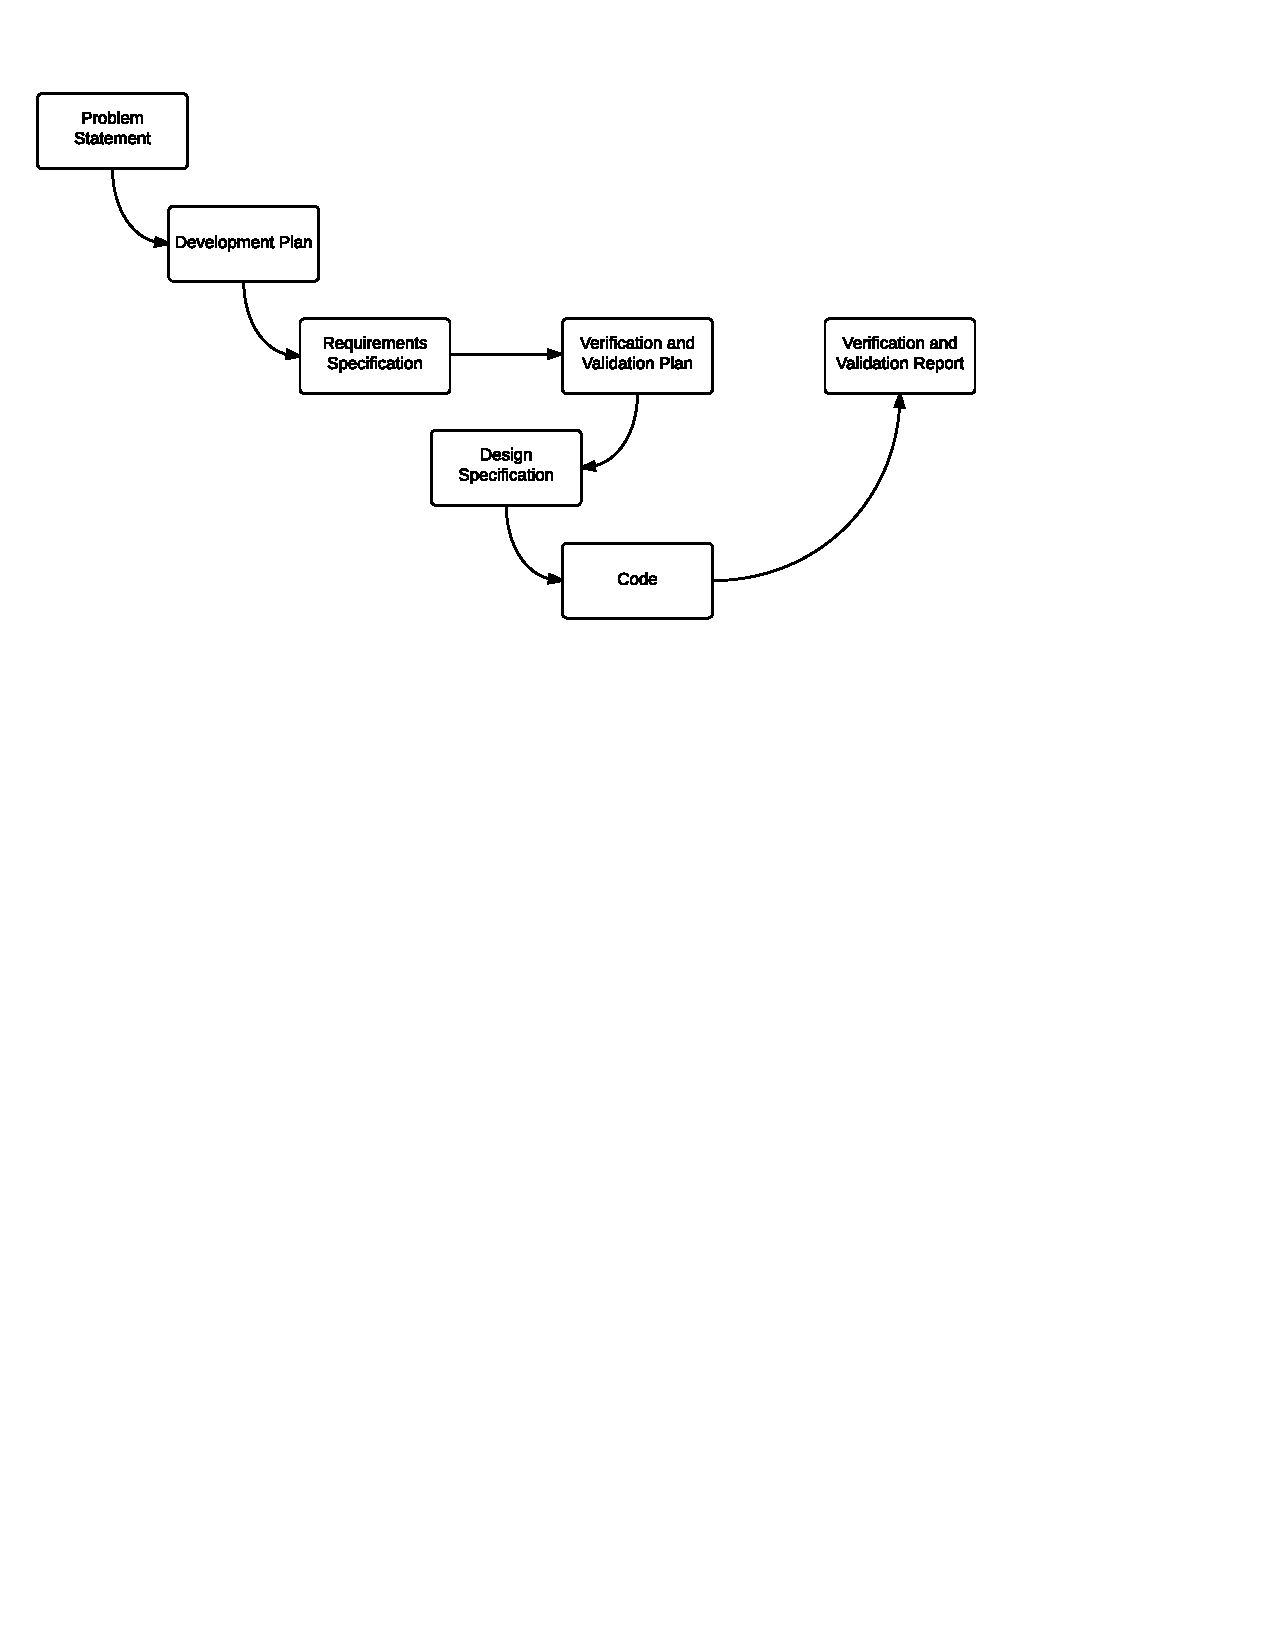
\includegraphics[scale=0.74]{OverviewOfProcess.pdf}
  \caption{The V-Model of Software Development \citep{smith5}}
\end{figure}

Grate is dedicated to writing high quality code through the application of 
strong software engineering principles. In order to meet that standard, the 
project will begin separated into 3 main stages. First, an extensive design and 
documentation phase before any part of the system is implemented. Once the 
project has been designed, then coding can commence. At the conclusion of 
coding, there will be an extensive testing and validation phase in order to 
build confidence in the functionality of the final product. The total time 
anticipated for this project is 4 months.

The design phase contains 6 deliverables: the problem statement, the development 
plan, the requirements specifications, the verification and validation plan, and 
the design specification. Creating the problem statement and the development 
plan should both take about 1 week. Creating the requirements specification, the 
verification and validation plan, and the design specification will all take 
about 2 weeks.

The coding phase involves implementing the project following the design 
specifications. The implementation of the project will take about 3 weeks.

Verification and Validation involves testing the project following the 
Verification and Validation Plan. The verification and validation of the project 
will take about 2 weeks.

Note that, despite the arrows in the diagram, this is an iterative process. This 
means that processes can happen more than once during the development process, 
with each iteration making improvements upon the previous iteration. Steps can 
also be skipped within iterations, or be performed out of order if deemed 
necessary. 

\subsubsection{Planning of the Development Phases}
This section is outlined in the development and design documents.

\subsection{Migration to the New Product}
This project requires no migration and therefore this is not applicable.

\subsection{Risks}

The external APIs used poses the most significant risk for Grate. APIs will be 
used to define core aspects of the models and the view of the project. That is, 
APIs will dictate the car entity in terms that can be used with many physics 
equations, which is important for calculating the fitness function of the car. 
In the event that the chosen APIs cease to function as expected, then alternate 
arrangements will have to be made in order to complete the project. 

\subsection{Costs}
There will be no cost at all as all of the materials used will be free.

\subsection{User Documentation and Training}

\subsubsection{User Documentation Requirements}
The following documents will be created for Grate's Genetic Cars:

\begin{enumerate}

\item{Problem Statement}

This document will detail the scope and purpose of the project. It will be 
referred to by current and future developers of the project, as well as future, 
currently undetermined, stakeholders. The document will initially be created by 
all members of Grate; however, the responsibility of maintaining the document 
will rest with the team lead.

\item{Development Plan}

This document will detail the development process for the project. It will be 
referred to by the current developers of the project in order to prepare for 
upcoming milestones, as well as future developers who want to know the process 
of creating the initial project. This document will initially be created by all 
members of Grate; however, the responsibility of maintaining the document will 
rest with the team lead.

\item{Requirements Specification}

This document will detail the requirements for the project. It shall be a living 
document that evolves as the requirements change. It will be referenced by the 
current developers of the project. The document will be created by all members 
of Grate, and the responsibility of maintaining this document will lie with all 
members of Grate. 

\item{Verification and Validation Plan}

This document will detail the test cases used in order to validate the project. 
It will be used by testers of the project in order to increase confidence in the 
code. The document will be created by all members of Grate; however, the 
responsibility of maintaining the document will rest with the Quantitative 
Testing Expert.

\item{Design Specification Document}

This document will document the internal workings of the code. It will be used 
by future developers who want to learn how the current system functions. The 
document will be created by all members of Grate, and the responsibility of 
maintaining this document will lie with all members of Grate.

\item{User Manual}

The user manual will detail the operation procedures for Grate's Genetic Cars. 
It will explain to the users of Grate's Genetic Cars all of the different 
functions that Genetic Cars supports, as well as the role that different 
parameters play in the Genetic Algorithm. This document will be created by all 
members of Grate; however, the responsibility of maintaining the document will 
rest with the theory expert.
\end{enumerate}

\subsubsection{Training Requirements}
No specific training beyond what is listed under assumptions will be required of 
the user.

\newpage

\subsection{Waiting Room}
\begin{reqbox}
%
\begin{tabular}{cc}
Requirement \#: 29 & Requirement Type: Functional \\
\end{tabular} \\
%
\textbf{Description:} Users shall be able to replay any previous generations.\\
\textbf{Rationale:}  This requirement will allow users to compare the 
performance of cars between generations.\\
\textbf{Originator:} Kelvin Lin\\
\textbf{Fit Criterion:} The user can elect to see graphical output of a previous 
generation's cars.\\
%  
\textbf{Supporting Materials:} JavaScript \\
\textbf{History:} Created October 11\textsuperscript{th}, 2016
%
\end{reqbox}

\begin{reqbox}
%
\begin{tabular}{cc}
Requirement \#: 30 & Requirement Type: Functional \\
\end{tabular} \\
%
\textbf{Description:} Users shall be able to skip to any future generation.\\
\textbf{Rationale:}  This requirement will allow users to compare the 
performance of cars between generations.\\
\textbf{Originator:} Kelvin Lin\\
\textbf{Fit Criterion:} The user can elect to see graphical output of a future 
generation's cars.\\
%  
\textbf{Supporting Materials:} JavaScript \\
\textbf{History:} Created October 11\textsuperscript{th}, 2016
%
\end{reqbox}

\begin{reqbox}
%
\begin{tabular}{cc}
Requirement \#: 31 & Requirement Type: Functional \\
\end{tabular} \\
%
\textbf{Description:} Users shall be able to seeds that generated the top 
\textit{st} cars. \\
\textbf{Rationale:}  This requirement will allow users to compare the 
performance of cars evolved from different starting points.\\
\textbf{Originator:} Kelvin Lin\\
\textbf{Fit Criterion:} The user can see a list of seeds that generated the top 
\textit{st} cars.\\
%  
\textbf{Supporting Materials:} JavaScript \\
\textbf{History:} Created October 11\textsuperscript{th}, 2016
%
\end{reqbox}

\subsection{Ideas for Solutions}
Please refer to 
\href{https://gitlab.cas.mcmaster.ca/linkk4/GrateBox/tree/master/Doc/Wireframes}{the 
ideas for solutions}.

\bibliographystyle{plainnat}

\bibliography{SRS}

\newpage

\section{Appendix}

%%This section has been added to the Volere template.  This is where you can 
%place additional information.

\subsection{List of Figures}

\subsection{Symbolic Parameters}

%Code Generated From http://www.tablesgenerator.com/#
\begin{table}[h!]
\centering
\label{LOF}
\begin{tabular}{ll}
Symbol & Definition \\
\textit{s} & The number of samples in a generation  \\
\textit{v} & The number of vectors in a car  \\
\textit{number\_of\_vertices} & The number of vertices formed by connecting 
vectors in a car model \\
\textit{r} & The radius of a wheel\\
\textit{min\_weight} & The minimum mass of a car\\
\textit{max\_weight} & The maximum mass of a car\\
\textit{max\_secs} & The maximum amount of time a car is allowed to stall in one 
spot\\
\textit{n} & The number of car statistics to display\\
\textit{mutation\_rate} & The rate at which genes mutate\\
\textit{max\_cars\_per\_gen} & The maximum number of cars in a given 
generation\\
\textit{st} & The top random seeds \\
\textit{t} & The number of parents in a generation\\
\textit{t\_max} & The maximum number of parents\\
\textit{t\_min} & The minimum number of parents\\
\end{tabular}
\caption{List of Figures}
\end{table}


\end{document}



